\documentclass[10pt]{article}
\usepackage{amsmath,textcomp,amssymb,geometry,graphicx,enumerate,tikz,algorithm,algpseudocode,pifont}
\usetikzlibrary{calc}
\usetikzlibrary{datavisualization}
\usetikzlibrary{datavisualization.formats.functions}


\textheight=9in
\textwidth=7in
\topmargin=-.75in
\oddsidemargin=-0.25in
\evensidemargin=-0.25in

\usepackage{listings}
\lstnewenvironment{codeblock}
    {\lstset{language=Python,
      showspaces=false,
      showtabs=false,
      breaklines=true,
      mathescape=true,
      showstringspaces=false,
      breakatwhitespace=true,
      commentstyle=\textit,
      keywordstyle=\textbf,
      basicstyle=\ttfamily,
      escapechar=`,
      moredelim={**[is][{\color{RoyalBlue}}]{\^^M\\beginsol}{\^^M\\endsol}},
      moredelim={[is][{\color{RoyalBlue}}]{\^^M\\beginexp}{\^^M\\endexp}},
    }}
    {}


\begin{document}
\section*{02/22/2016}
	\subsection*{Anisotropic Multivariate Gaussians}
		\
		\begin{itemize}
			\item $X \sim \mathcal{N}(\mu, \Sigma) \Leftarrow X$ is random d-vector with mean $\mu$.
				\begin{align*}
					P(x) &= \frac{1}{\sqrt{(2\pi)^{d}}\sqrt{|\Sigma|}}\text{exp}(-\frac{1}{2}(x-\mu)^{T}\Sigma^{-1}(x-\mu))
				\end{align*}
			\item $\Sigma$ is the $d$x$d$ SPD \underline{covariance matrix}
			\item $\Sigma^{-1}$ is the $d$x$d$ SPD \underline{precision matrix}; serves as a metric tensor.
			\item Write $P(x) = n(q(x))$, where $q(x) = (x-\mu)^{T}\Sigma^{-1}(x-\mu)$. Note, $n: \mathbb{R} \rightarrow \mathbb{R}$, exponential, $q: \mathbb{R}^{d} \rightarrow \mathbb{R}$, quadratic.
			\item Principle: given $f: \mathbb{R} \rightarrow \mathbb{R}$, isosurfaces of $f(q(x))$ are same as $q(x)$ (different isovalues), except that some might be "combined."
				\begin{center}
					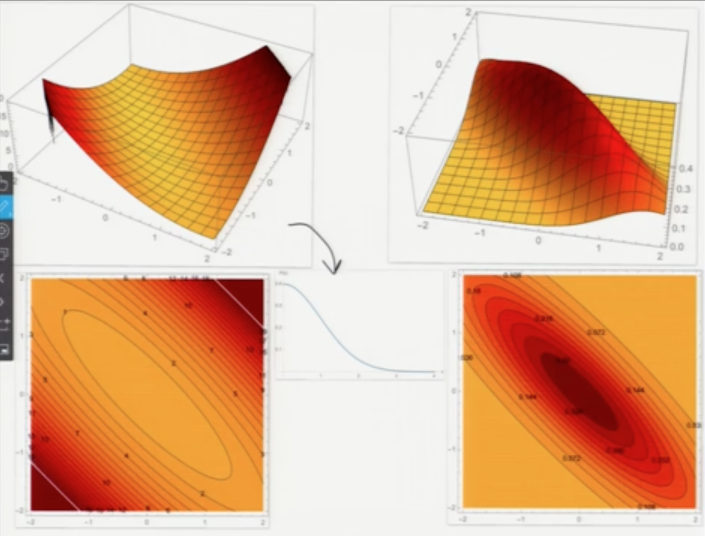
\includegraphics[scale=0.5]{../images/gaussiantransformation}
				\end{center}
			\item \underline{Covariance}:
				\begin{align*}
					\text{Cov}(X, Y) &= E[(X - E[X])(Y - E[Y])^{T}]\\
									&= E[XY^{T}] - \mu_{x}\mu_{y}^{T}\\
					\text{Var}(X) &= \text{Cov}(X, X)\\
				\end{align*}
				\begin{itemize}
					\item For a Gaussian, one can show Var($X$) = $\Sigma$. Hence,
						\begin{align*}
							\Sigma =
								\begin{bmatrix}
									\text{Var}(X_{1}) & \text{Cov}(X_{1},X_{2}) & \dots & \text{Cov}(X_{1},X_{d})\\
									\text{Cov}(X_{2},X_{1})  & \text{Var}(X_{2}) & \dots & \text{Cov}(X_{2}, X_{d})\\
									\vdots & & \ddots & \vdots &\\
									\text{Cov}(X_{d},X_{1}) & \text{Cov}(X_{d},X_{2}) & \dots & \text{Var}(X_{d})\\
								\end{bmatrix}
						\end{align*}	
					\item $X_{i}, X_{j}$ independent $\Rightarrow$ Cov($X_{i}, X_{j}$) = 0.
					\item Cov($X_{i}, X_{j}$) = 0 and they come from a joint normal distribution $\Rightarrow X_{i}, X_{j}$ independent.
					\item All features pairwise independent $\Rightarrow \Sigma$ is diagonal.
						\begin{align*}
							\Sigma \ \text{is diagonal} &\Leftrightarrow \text{axis-aligned Gaussian; squared radii on the diagonal}.\\
							&\Leftrightarrow P(x) = P(X_{1})P(X_{2}) \dots P(X_{d})\\
						\end{align*}

\begin{center}						
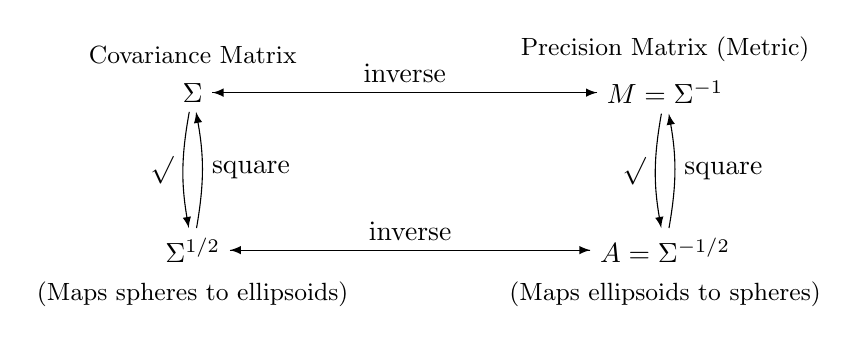
\begin{tikzpicture}
[ar/.style={->,thick},no/.style={}]
\node [no][label={\small Covariance Matrix}] at (0cm,4cm) (A) {$\Sigma$};
\node [no][label={\small Precision Matrix (Metric)}] at (6cm,4cm) (B) {$M = \Sigma^{-1}$};
\node [no][label=below:{\small (Maps ellipsoids to spheres)}] at (6cm,2cm) (D) {$A=\Sigma^{-1/{2}}$};
\node [no][label=below:{\small (Maps spheres to ellipsoids)}] at (0cm,2cm) (E) {$\Sigma^{1/{2}}$};

\draw [-latex] (A) -- node[above] {inverse} (B);
\draw [-latex] (B) -- node[above] {} (A);

\draw [-latex] (A) to[bend right=10] node[left] {$\sqrt{}$} (E);
\draw [-latex] (E) to[bend right=10] node[right] {square} (A);

\draw [-latex] (B) to[bend right=10] node[left] {$\sqrt{}$} (D);
\draw [-latex] (D) to[bend right=10] node[right] {square} (B);


\draw [-latex] (D) -- node[above] {inverse} (E);
\draw [-latex] (E) -- node[above] {} (D);
\end{tikzpicture}
\end{center}	
					\item Eigenvalues of $\Sigma^{1/{2}}$ are ellipsoid radii (standard deviations along the eigenvectors).
					\item Eigenvalues of $\Sigma$ are variances along along eigenvectors.
					\item Diagonalizing $\Sigma = V\Lambda V^{T}$, $\Sigma^{\frac{1}{2}} = V\Lambda^{\frac{1}{2}}V^{T}$.
				\end{itemize}
			\end{itemize}
		
		\subsection*{Maximum Likelihood estimation for anisotropic Gaussians}
			\
			\begin{itemize}
				\item Given samples $x_{1}, \dots, x_{n}$ and classes $y_{1}, \dots y_{n}$ find the best-fit Gaussians.
				\item For QDA:
					\begin{align*}
						\hat{\Sigma_{c}} = \frac{1}{n_{c}} \sum_{i:y_{i}=c} (x_{i} - \mu_{c})(x_{i} - \mu_{c})^{T} \Leftarrow \text{conditional covariance for samples in class c}
					\end{align*}
					\begin{center}
						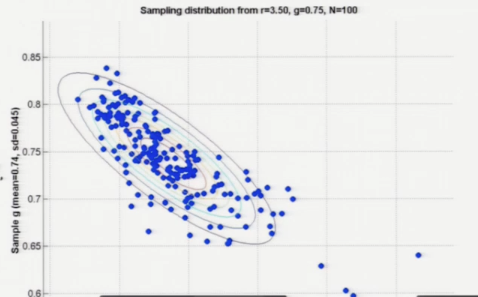
\includegraphics[scale=0.5]{../images/smaple}
					\end{center}
					\begin{itemize}
					\item Priors $\pi_{c}$ and means $\hat{\mu_{c}}$ same as before.
					\item $\hat{\Sigma_{c}}$ is the positive semidefinite. If some zero eigenvalue, must eliminate the zero-variance dimension.
					\end{itemize}
				\item For LDA:
					\begin{align*}
						\hat{\Sigma} = \frac{1}{n} \sum_{c} \sum_{i:y_{i}=c} (x_{i} - \mu_{c})(x_{i} - \mu_{c})^{T} \Leftarrow \text{pooled within class covariance matrix}
					\end{align*}
				\item \underline{QDA}:
					\begin{itemize}
						\item $\pi_{c}, \mu_{c}, \Sigma_{c}$ may be different for each class c.
						\item Goal is to choose c that maximizes $P(X=x|Y=c)\pi_{c}$ , which is equivalent to maximizing the \underline{quadratic discriminant function},
							\begin{align*}
								Q_{c}(x) &= \ln \Big(\sqrt{(2\pi)^{d}}P(x)\pi_{c}\Big)\\
										&= -\frac{1}{2}q_{c}(x)-\frac{1}{2} \ln |\Sigma_{c}| + \ln \pi_{c}
							\end{align*}
						\item 2 classes: Prediction function $Q_{c}(x) - Q_{d}(x)$ is quadratic, but may be indefinite.
						\item Since the prediction function is quadratic $\Rightarrow$ Bayes decision boundary is quadric.
						\item Posterior is $P(Y=c|X=x) = s(Q_{c}(x) - Q_{d}(x))$ where $s(\cdot)$ is the logistic function.
							\begin{center}
								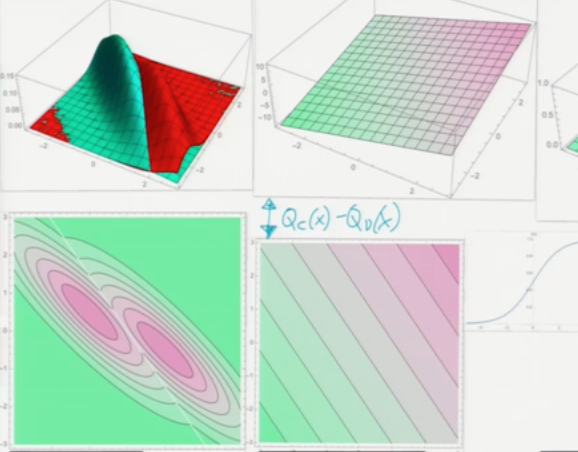
\includegraphics[scale=0.5]{../images/LDA}
							\end{center} 
					\end{itemize}
				
				\item \underline{LDA}:
					\begin{itemize}
						\item Once $\Sigma$ for all classes.
							\begin{align*}
								Q_{c}(x) - Q_{d}(x) &= (\mu_{c} - \mu_{d})^{T} \Sigma^{-1}x - \frac{\mu_{c}^{T}\Sigma^{-1}\mu_{c} - \mu_{d}^{T}\Sigma^{-1}\mu_{d}}{2} + \ln \pi_{c} - \ln \pi_{d}
							\end{align*}
						\item Choose class c that maximizes the \underline{linear discriminant function},
							\begin{align*}
								\mu^{T}\Sigma^{-1}x - \frac{1}{2}\mu_{c}^{T}\Sigma^{-1}\mu_{c} + \ln \pi_{c}
							\end{align*}
						\item 2 classes:
							\begin{itemize}
								\item Decision boundary is $w^{T}x + \alpha = 0$
								\item Posterior is $P(Y=c|X=x) = s(w^{T}x + \alpha)$.
							\end{itemize}
							\begin{center}
								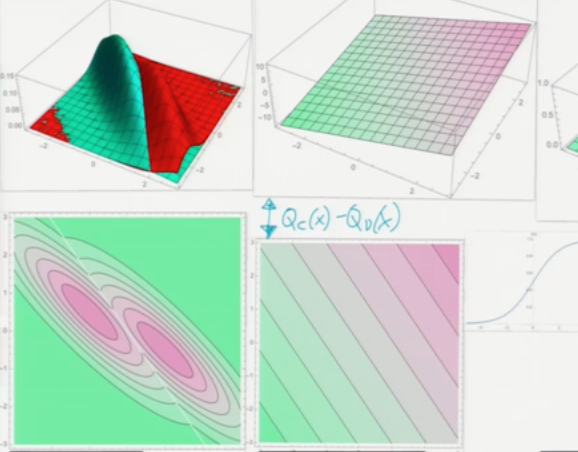
\includegraphics[scale=0.5]{../images/LDA}
							\end{center}
					\end{itemize}
				\item \underline{Notes}
					\
					\begin{itemize}
						\item Changing prior $\pi_{c}$ (or loss) is easy: if its LDA adjust $\alpha$.
						\item LDA is often interpreted as projecting samples onto the normal vector.
							\begin{center}
								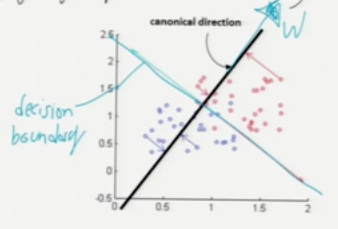
\includegraphics[scale=0.5]{../images/lda_projections}
							\end{center}
						\item For 2 classes,
							\begin{itemize}
								\item LDA has $d + 1$ parameters ($w, \alpha$).
								\item QDA has $\frac{d(d+3)}{2} + 1$ parameters
								\item $\Rightarrow$ QDA more likely to overfit.
							\end{itemize}
							\begin{center}
								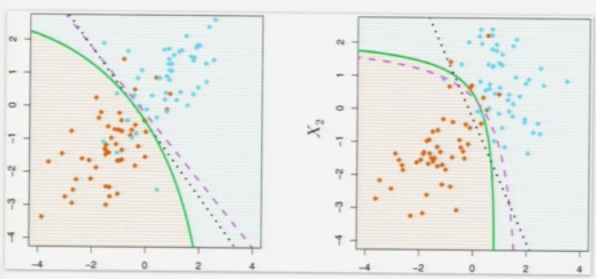
\includegraphics[scale=0.5]{../images/overfitting}
							\end{center}
					\end{itemize}
			\end{itemize}
\end{document}
